\begin{apendicesenv}

% Imprime uma página indicando o início dos apêndices
\partapendices

% =====================================================================================================
% ============================================= Chapter ===============================================
% =====================================================================================================
\chapter{Códigos-fonte}
\label{ch:codigos_extras}

\section{Método de pesquisa em grade}

\lstinputlisting[	
	caption={Pesquisa em grade com número escalar},
	captionpos=t,
	label={lst:grid_search_scalar},
	language=Python,
	style=Python_lang]
	{./4_Codes/grid_search_scalar.py}
	\begin{center}
		\makebox[\width]{Fonte: Autor, adaptado de \citeonline{Haugen2018}}
	\end{center}

\section{Método de pesquisa em grade com duas variáveis}

\lstinputlisting[	
	caption={Pesquisa em grade com duas variáveis},
	captionpos=t,
	label={lst:grid_search_vectorial},
	language=Python,
	style=Python_lang]
	{./4_Codes/grid_search_vectorial.py}
	\begin{center}
		\makebox[\width]{Fonte: Autor, adaptado de \citeonline{Haugen2018}}
	\end{center}

\section{Exemplo do método \acrlong{mhe}}

% (Brincalepe): O código da página 44 deve ser deslocado para o apêndice.
% (cont.) Se quiser, destaque apenas alguma parte mais relevante e mantenha no corpo do texto.
\lstinputlisting[	
	caption={Exemplo do método \acrlong{mhe}},
	captionpos=t,
	label={lst:mhe_example},
	language=Python,
	style=Python_lang]
	{./4_Codes/mhe_example.py}
	\begin{center}
		\makebox[\width]{Fonte: Autor, adaptado de \citeonline{Haugen2018}}
	\end{center}

\section{Exemplo de aplicação do \acrlong{mpc}}

\lstinputlisting[	
	caption={Exemplo de aplicação do \acrlong{mpc}},
	captionpos=t,
	label={lst:mpc_example},
	language=Python,
	style=Python_lang]
	{./4_Codes/mpc_example.py}
	\begin{center}
		\makebox[\width]{Fonte: Autor, adaptado de \citeonline{Haugen2018}}
	\end{center}
% (Brincalepe): O código da página 58 também pode ser deslocado para o Apêndice.
% (cont.) Seria interessante descrevê-lo no corpo de texto através de um diagrama.

\section{Criação de diversos modelos experimentais do \acrshort{tclabsp}}
\label{sec:tclabsp-models-creation}

\lstinputlisting[	
	caption={Criação de diversos modelos experimentais do \acrshort{tclabsp}},
	captionpos=t,
    label={lst:tclabsp-models-creation},
    firstline=56,
    lastline=387,
    language=Matlab,
	style=Matlab_lang]
	{D:/Repos/TCLabSP/Simulink (MATLAB R2016a)/02-ModeloExperimental/RunMe.m}
	\begin{center}
		\makebox[\width]{Fonte: Autor}
    \end{center}
% TODO: Substituir endereço do arquivo

% =====================================================================================================
% ============================================= Chapter ===============================================
% =====================================================================================================
\chapter{Escolha da frequência de amostragem utilizando autocovariância}
\label{ch:sampling_time_using_autocorrelation}

A regra prática para a escolha da frequência de amostragem de sinal descrita por \citeonline{Aguirre2015}
e citada na \cref{subsubsec:periodo_de_amostragem} pode nem sempre ajudar muito, uma vez que é possível
que não se tenha nenhum conhecimento prévio do sinal para poder aplicar a regra de escolher uma frequência
de 5 a 10 vezes maior que a frequência de interesse \cite{Aguirre2015}. Para casos assim, \citeonline{Aguirre2015}
descreve uma outra técnica, que será apresentada nos parágrafos a seguir. 

Assume-se que o sinal já amostrado, $y^*(k)$, tenha sido obtido utilizando-se um tempo
de amostragem muito pequeno, ou seja, o sinal está superamostrado. Sendo assim, deseja-se encontrar o
valor $\Delta$ que descreva a fração pela qual o $y^*(k)$ pode ser decimado a fim de obter um sinal de trabalho
$y(k) = y^*(\Delta k)$, ou seja, o sinal decimado que ainda mantem as características originais do sinal $y^*(k)$.

Para fazer isso é necessário verificar o nível de correlação entre observações adjacentes do sinal
$y^*(k)$. Quanto mais superamostrado estiver o sinal $y^*(k)$, maior será a redundância entre duas
observações consecutivas. Este nível de correlação pode ser obtido calculando as funções de
autocovariância linear e não-linear (mostradas na \cref{eq:autocorrelation}) do sinal original.

\begin{subequations}
    \label{eq:autocorrelation}
    \begin{align}
		r_{y^*}(\tau) &= \mathrm{E} \left[(y^*(k) - \overline{y^*(k)}) (y^*(k - \tau) - \overline{y^*(k)})\right]		\\
		r_{y^{*2'}}(\tau) &= \mathrm{E} \left[(y^{*2}(k) - \overline{y^{*2}(k)}) (y^{*2}(k - \tau) - \overline{y^{*2}(k)})\right]
    \end{align}
\end{subequations}

$\mathrm{E}[\cdot]$ indica a esperança matemática, porém, sendo $y^*(k)$ ergótico, $\mathrm{E}[\cdot]$
pode ser substituída pela média temporal.

Após calculados $r_{y^*}(\tau)$ e $r_{y^{*2'}}(\tau)$, determinam-se seus primeiros mínimos,
$\tau_{y^*}$ e $\tau_{y^{*2'}}$, respectivamente. O menor desses mínimos passa a ser o valor de trabalho
$\tau_{m}^{*}$, ou seja, $\tau_{m}^{*} = \mathrm{min} \left[ \tau_{y^*} , \tau_{y^{*2'}} \right]$.

Por fim, deseja-se escolha $\Delta$ de forma que as funções de autocovariância do sinal decimado $y(k) = y^*(k)$
satisfaçam

\begin{equation}
    \label{eq:tau_m}
    10 \leq \tau_m \leq 20
\end{equation}

\noindent
sendo que $\tau_m$ é definido pelo sinal decimado $y(k)$ de maneira análoga a $\tau_m^*$ para o
sinal $y^*(k)$. Os limites inferior e superior da \cref{eq:tau_m} podem ser relaxados para
$5$ e $10$, respectivamente.

% =====================================================================================================
% ============================================= Section ===============================================
% =====================================================================================================
\section{Aplicação prática}
\label{ch:using_sampling_time_with_autocorrelation}

As \cref{fig:rise_time_sensor1,fig:rise_time_sensor2} da \cref{subsubsec:periodo_de_amostragem}
apresentam a resposta dos sensores de temperatura do \acrshort{tclabsp} quando o Aquecedor 1 é
excitado com um degrau de 0 à 50\%.

Após alguns testes preliminares, foi observado que o sistema apresentava uma resposta lenta
e que, portanto, uma coleta de dados com tempo de amostragem de $0.25s$ seria suficiente para
superamostrar os dados e garantir que todas as características de resposta do sistema tenham
sido amostradas.

Calcula-se então as funções de autocovariância apresentadas na \cref{eq:autocorrelation} para os
sensores de temperatura 1 e 2, como apresentado na \cref{fig:autocorrelationS1S2}.

\begin{figure}[h]
	\caption{Funções de autocovariância dos Sensores de Temperatura 1 e 2}
	\begin{center}
		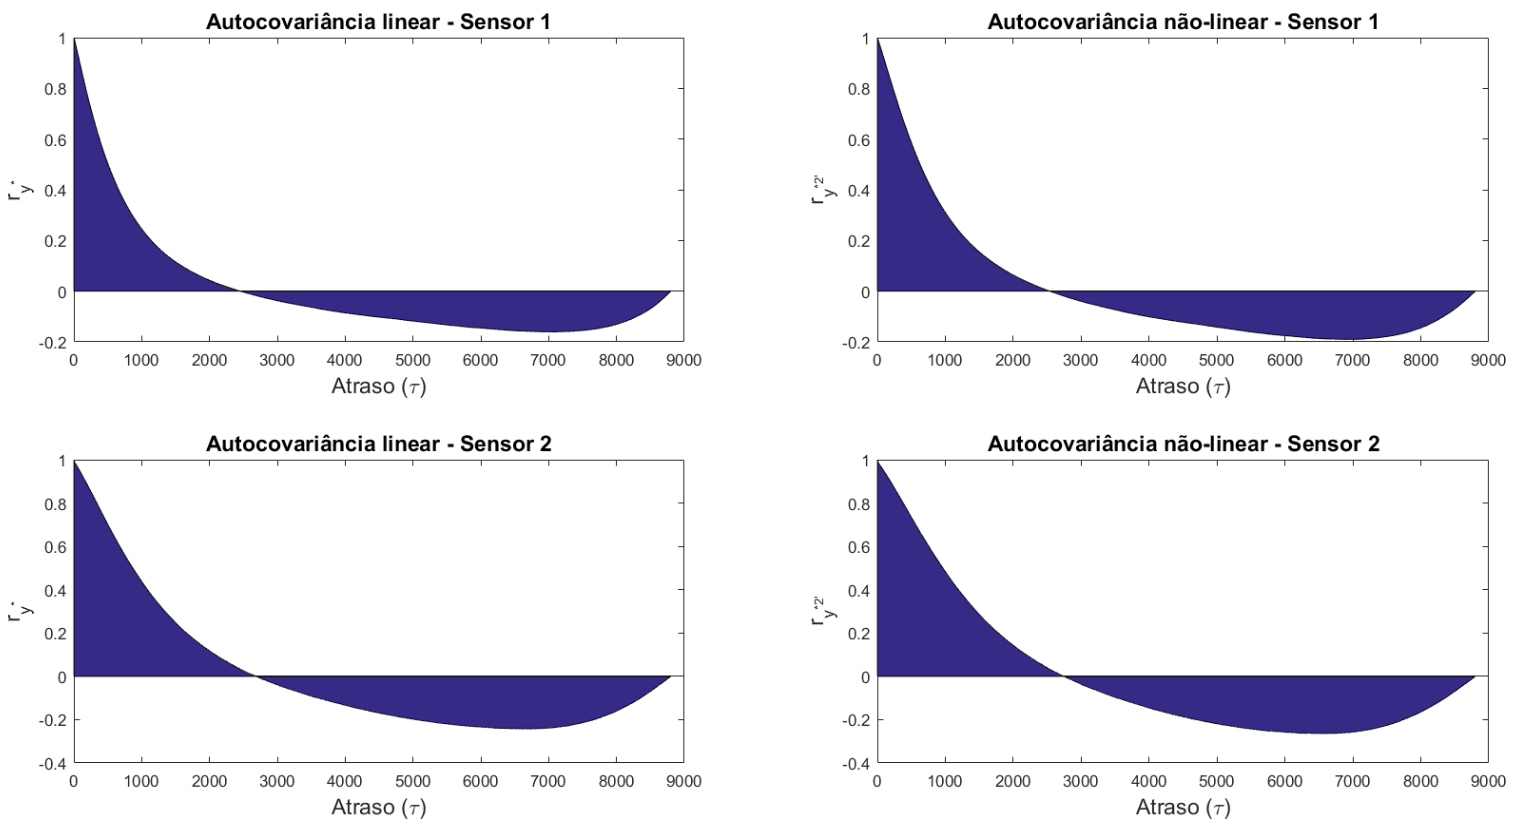
\includegraphics[width=0.95\textwidth]{./5_images/AutocorrelationS1S2.png} 
		\label{fig:autocorrelationS1S2}
	\end{center}
	\centering
	\makebox[\width]{Fonte: \citeonline{Prata2019}} 
\end{figure}

Para cada um dos sensores, encontramos então o valor mínimo das funções de autocovariância
($\tau_{y^{*}}$ e $\tau_{y^{*2'}}$), e a partir delas determinamos $\tau_m^*$
($\tau_{m}^{*} = \mathrm{min} \left[ \tau_{y^*} , \tau_{y^{*2'}} \right]$).
O resultado é apresentado na \cref{tab:tau_s1s2}.

\begin{table}[h]
	\centering
	\caption{Mínimos das funções de autocovariância}
	\label{tab:tau_s1s2}
	\begin{tabular}{llll} \toprule
		{Sensor}		& {$\tau_{y^{*}}$}		& {$\tau_{y^{*2'}}$}		& {$\pmb{\tau}_{\pmb{m}}^{\pmb{*}}$}		\\ \midrule
		Sensor 1		& $7015$				& $6925$					& $\pmb{6}\pmb{9}\pmb{2}\pmb{5}$			\\
		Sensor 2		& $6735$				& $6621$					& $\pmb{6}\pmb{6}\pmb{2}\pmb{1}$			\\ \bottomrule
	\end{tabular}
	\caption*{Fonte: Autor}
\end{table}

Conhecendo $\tau_{m}^{*}$ é possível encontrar um valor de $\Delta$ para obter o sinal decimado
$y(k) = y^*(\Delta k)$, tal que o valor mínimo da suas funções de autocovariância satisfaçam
\cref{eq:tau_m}.

Uma demonstração do efeito da variação do $\Delta$ no tempo de amostragem do sinal
pode ver vista na \cref{tab:delta_action}

\begin{table}[h]
	\centering
	\caption{Efeito do $\Delta$ no tempo de amostragem}
	\label{tab:delta_action}
	\begin{tabular}{cccccc} \toprule
		{k}			& {$\Delta=1$}		& {$\Delta=2$}		& {$\cdots$}	& {$\Delta=4$}	& {$\cdots$} 	\\ \midrule
		1			& $0.00$			& $0.00$			& \hfill		& $0.00$		& \hfill		\\
		2			& $0.25$			& $0.50$			& \hfill		& $1.00$		& \hfill		\\
		3			& $0.50$			& $1.00$			& \hfill		& $2.00$		& \hfill		\\
		4			& $0.75$			& $0.50$			& \hfill		& $3.00$		& \hfill		\\
		5			& $1.00$			& $2.00$			& \hfill		& $4.00$		& \hfill		\\ 
		$\vdots$	& $\vdots$			& $\vdots$			& \hfill		& $\vdots$		& \hfill		\\ \bottomrule 
	\end{tabular}
	\caption*{Fonte: Autor}
\end{table}

Através de um algoritmo\footnote{
	Indicar algoritmo utilizado			% TODO Indicar algoritmo utilizado
} foi possível testar diferentes valores de $\Delta$ a fim de encontrar
aquele que primeiro satisfizesse a \cref{eq:tau_m}, e por meio deste algoritmo encontrou-se
os valores de $\Delta$ e de $T_s$ (tempo de amostragem) indicados da \cref{eq:delta_and_ts}.

\begin{subequations}
    \label{eq:delta_and_ts}
    \begin{align}
		\Delta &= 253	\\
		T_s &= 63.25s
    \end{align}
\end{subequations}


\end{apendicesenv}